%  LaTeX support: latex@mdpi.com 
%  For support, please attach all files needed for compiling as well as the log file, and specify your operating system, LaTeX version, and LaTeX editor.

%=================================================================
\documentclass[journal,article,submit,pdftex,moreauthors]{Definitions/mdpi} 
%--------------------
% Class Options:
%--------------------
%----------
% journal
%----------
% Choose between the following MDPI journals:
% acoustics, actuators, addictions, admsci, adolescents, aerobiology, aerospace, agriculture, agriengineering, agrochemicals, agronomy, ai, air, algorithms, allergies, alloys, analytica, analytics, anatomia, animals, antibiotics, antibodies, antioxidants, applbiosci, appliedchem, appliedmath, applmech, applmicrobiol, applnano, applsci, aquacj, architecture, arm, arthropoda, arts, asc, asi, astronomy, atmosphere, atoms, audiolres, automation, axioms, bacteria, batteries, bdcc, behavsci, beverages, biochem, bioengineering, biologics, biology, biomass, biomechanics, biomed, biomedicines, biomedinformatics, biomimetics, biomolecules, biophysica, biosensors, biotech, birds, bloods, blsf, brainsci, breath, buildings, businesses, cancers, carbon, cardiogenetics, catalysts, cells, ceramics, challenges, chemengineering, chemistry, chemosensors, chemproc, children, chips, cimb, civileng, cleantechnol, climate, clinpract, clockssleep, cmd, coasts, coatings, colloids, colorants, commodities, compounds, computation, computers, condensedmatter, conservation, constrmater, cosmetics, covid, crops, cryptography, crystals, csmf, ctn, curroncol, cyber, dairy, data, ddc, dentistry, dermato, dermatopathology, designs, devices, diabetology, diagnostics, dietetics, digital, disabilities, diseases, diversity, dna, drones, dynamics, earth, ebj, ecologies, econometrics, economies, education, ejihpe, electricity, electrochem, electronicmat, electronics, encyclopedia, endocrines, energies, eng, engproc, entomology, entropy, environments, environsciproc, epidemiologia, epigenomes, est, fermentation, fibers, fintech, fire, fishes, fluids, foods, forecasting, forensicsci, forests, foundations, fractalfract, fuels, future, futureinternet, futurepharmacol, futurephys, futuretransp, galaxies, games, gases, gastroent, gastrointestdisord, gels, genealogy, genes, geographies, geohazards, geomatics, geosciences, geotechnics, geriatrics, grasses, gucdd, hazardousmatters, healthcare, hearts, hemato, hematolrep, heritage, higheredu, highthroughput, histories, horticulturae, hospitals, humanities, humans, hydrobiology, hydrogen, hydrology, hygiene, idr, ijerph, ijfs, ijgi, ijms, ijns, ijpb, ijtm, ijtpp, ime, immuno, informatics, information, infrastructures, inorganics, insects, instruments, inventions, iot, j, jal, jcdd, jcm, jcp, jcs, jcto, jdb, jeta, jfb, jfmk, jimaging, jintelligence, jlpea, jmmp, jmp, jmse, jne, jnt, jof, joitmc, jor, journalmedia, jox, jpm, jrfm, jsan, jtaer, jvd, jzbg, kidneydial, kinasesphosphatases, knowledge, land, languages, laws, life, liquids, literature, livers, logics, logistics, lubricants, lymphatics, machines, macromol, magnetism, magnetochemistry, make, marinedrugs, materials, materproc, mathematics, mca, measurements, medicina, medicines, medsci, membranes, merits, metabolites, metals, meteorology, methane, metrology, micro, microarrays, microbiolres, micromachines, microorganisms, microplastics, minerals, mining, modelling, molbank, molecules, mps, msf, mti, muscles, nanoenergyadv, nanomanufacturing,\gdef\@continuouspages{yes}} nanomaterials, ncrna, ndt, network, neuroglia, neurolint, neurosci, nitrogen, notspecified, %%nri, nursrep, nutraceuticals, nutrients, obesities, oceans, ohbm, onco, %oncopathology, optics, oral, organics, organoids, osteology, oxygen, parasites, parasitologia, particles, pathogens, pathophysiology, pediatrrep, pharmaceuticals, pharmaceutics, pharmacoepidemiology,\gdef\@ISSN{2813-0618}\gdef\@continuous pharmacy, philosophies, photochem, photonics, phycology, physchem, physics, physiologia, plants, plasma, platforms, pollutants, polymers, polysaccharides, poultry, powders, preprints, proceedings, processes, prosthesis, proteomes, psf, psych, psychiatryint, psychoactives, publications, quantumrep, quaternary, qubs, radiation, reactions, receptors, recycling, regeneration, religions, remotesensing, reports, reprodmed, resources, rheumato, risks, robotics, ruminants, safety, sci, scipharm, sclerosis, seeds, sensors, separations, sexes, signals, sinusitis, skins, smartcities, sna, societies, socsci, software, soilsystems, solar, solids, spectroscj, sports, standards, stats, std, stresses, surfaces, surgeries, suschem, sustainability, symmetry, synbio, systems, targets, taxonomy, technologies, telecom, test, textiles, thalassrep, thermo, tomography, tourismhosp, toxics, toxins, transplantology, transportation, traumacare, traumas, tropicalmed, universe, urbansci, uro, vaccines, vehicles, venereology, vetsci, vibration, virtualworlds, viruses, vision, waste, water, wem, wevj, wind, women, world, youth, zoonoticdis 
% For posting an early version of this manuscript as a preprint, you may use "preprints" as the journal. Changing "submit" to "accept" before posting will remove line numbers.

%---------
% article
%---------
% The default type of manuscript is "article", but can be replaced by: 
% abstract, addendum, article, book, bookreview, briefreport, casereport, comment, commentary, communication, conferenceproceedings, correction, conferencereport, entry, expressionofconcern, extendedabstract, datadescriptor, editorial, essay, erratum, hypothesis, interestingimage, obituary, opinion, projectreport, reply, retraction, review, perspective, protocol, shortnote, studyprotocol, systematicreview, supfile, technicalnote, viewpoint, guidelines, registeredreport, tutorial
% supfile = supplementary materials

%----------
% submit
%----------
% The class option "submit" will be changed to "accept" by the Editorial Office when the paper is accepted. This will only make changes to the frontpage (e.g., the logo of the journal will get visible), the headings, and the copyright information. Also, line numbering will be removed. Journal info and pagination for accepted papers will also be assigned by the Editorial Office.

%------------------
% moreauthors
%------------------
% If there is only one author the class option oneauthor should be used. Otherwise use the class option moreauthors.

%---------
% pdftex
%---------
% The option pdftex is for use with pdfLaTeX. Remove "pdftex" for (1) compiling with LaTeX & dvi2pdf (if eps figures are used) or for (2) compiling with XeLaTeX.

%=================================================================
% MDPI internal commands - do not modify
\firstpage{1} 
\makeatletter 
\setcounter{page}{\@firstpage} 
\makeatother
\pubvolume{1}
\issuenum{1}
\articlenumber{0}
\pubyear{2024}
\copyrightyear{2024}
%\externaleditor{Academic Editor: Firstname Lastname}
\datereceived{ } 
\daterevised{ } % Comment out if no revised date
\dateaccepted{ } 
\datepublished{ } 
%\datecorrected{} % For corrected papers: "Corrected: XXX" date in the original paper.
%\dateretracted{} % For corrected papers: "Retracted: XXX" date in the original paper.
\hreflink{https://doi.org/} % If needed use \linebreak
%\doinum{}
%\pdfoutput=1 % Uncommented for upload to arXiv.org
%\CorrStatement{yes}  % For updates


%=================================================================
% Add packages and commands here. The following packages are loaded in our class file: fontenc, inputenc, calc, indentfirst, fancyhdr, graphicx, epstopdf, lastpage, ifthen, float, amsmath, amssymb, lineno, setspace, enumitem, mathpazo, booktabs, titlesec, etoolbox, tabto, xcolor, colortbl, soul, multirow, microtype, tikz, totcount, changepage, attrib, upgreek, array, tabularx, pbox, ragged2e, tocloft, marginnote, marginfix, enotez, amsthm, natbib, hyperref, cleveref, scrextend, url, geometry, newfloat, caption, draftwatermark, seqsplit
% cleveref: load \crefname definitions after \begin{document}
\usepackage{xcolor}
\usepackage[style=numeric,sorting=none]{biblatex} %Imports biblatex package
\addbibresource{Bibliography.bib} %Import the bibliography file
\usepackage{longtable}
%=================================================================
% Please use the following mathematics environments: Theorem, Lemma, Corollary, Proposition, Characterization, Property, Problem, Example, ExamplesandDefinitions, Hypothesis, Remark, Definition, Notation, Assumption
%% For proofs, please use the proof environment (the amsthm package is loaded by the MDPI class).

%=================================================================
% Full title of the paper (Capitalized)
\Title{Calorie Restriction and Time-Restricted Feeding: effective interventions in overweight or obese patients undergoing radiotherapy treatment with curative intent for cancer.}

% MDPI internal command: Title for citation in the left column
\TitleCitation{Title}

% Authors, for the paper (add full first names)
\Author{Carmen Vega$^{1}$, Esteban Barnafi$^{2}$, César Sánchez$^{3}$, Francisco Acevedo$^{3}$, Benjamin Walbaum$^{3}$, Alejandra Parada$^{4}$, Nicolás Rivas$^{2}$, and Tomás Merino$^{1,}*$}

%\longauthorlist{yes}

% MDPI internal command: Authors, for metadata in PDF
\AuthorNames{Firstname Lastname, Firstname Lastname and Firstname Lastname}

% MDPI internal command: Authors, for citation in the left column
\AuthorCitation{Lastname, F.; Lastname, F.; Lastname, F.}
% If this is a Chicago style journal: Lastname, Firstname, Firstname Lastname, and Firstname Lastname.

% Affiliations / Addresses (Add [1] after \address if there is only one affiliation.)
\address{%
$^{1}$ \quad Cancer Center UC, Red de Salud Christus-UC, Santiago 8330032, Chile\\
$^{2}$ \quad Faculty of Medicine, Pontificia Universidad Católica de Chile, Santiago 8331150, Chile\\
$^{3}$ \quad Department of Hematology-Oncology, Faculty of Medicine, Pontificia Universidad Católica de Chile, Santiago 8330077, Chile\\
$^{4}$ \quad Department of Health Sciences, Nutrition and Dietetics Program, Faculty of Medicine, Pontificia Universidad Católica de Chile, Santiago 78204360, Chile
}
% Contact information of the corresponding author
\corres{Correspondence: tomasmerinolara@gmail.com}

% Abstract (Do not insert blank lines, i.e. \\) 

\abstract{This study assesses the feasibility of Calorie Restriction (CR) and Time-Restricted Feeding (TRF) in overweight and obese cancer patients, who realized little to no physical activity, undergoing curative radiotherapy, structured as a prospective, interventional, non-randomized {\color{blue}open label} clinical trial. Of the 27 participants initially enrolled, 21 patients with breast cancer were selected for analysis. Participants self-selected into two dietary interventions: TRF, comprising a sugar and saturated fat-free diet calibrated to individual energy needs, consumed within an 8-hour eating window followed by a 16-hour fast; or CR, involving a 25\% reduction in total caloric intake from energy expenditure, distributed across 4 meals and 1 snack with 55\% carbohydrates, 15\% protein, and 30\% fats, excluding sugars and saturated fats. The primary goal was to evaluate the feasibility of these diets in the specific patient group. Results indicate that both interventions are effective and statistically significant for weight loss and reducing waist circumference, with TRF showing a stronger impact in this study. Changes in LDL, HDL, Total Cholesterol, Triglycerides, Glucose and Insulin were not statistically significant.}

% Keywords
\keyword{Intermittent Fasting, Cancer, Curative, Radiotherapy, Calorie Restriction, Time-Restricted Feeding, Diet, Nutrition, Overweight, Obesity} 

%%%%%%%%%%%%%%%%%%%%%%%%%%%%%%%%%%%%%%%%%%
\begin{document}

%%%%%%%%%%%%%%%%%%%%%%%%%%%%%%%%%%%%%%%%%%
% The order of the section titles is different for some journals. Please refer to the "Instructions for Authors” on the journal homepage.

\section{Introduction}

In the last decade, cancer and cardiovascular diseases have established themselves as the first cause of morbidity and mortality collectively, with over 18 million new cases of cancer being registered only in 2020 \cite{cancertoday}. These pathologies share common risk factors such as sedentary lifestyle, poor diet, obesity, tobacco and alcohol consumption \cite{WHOtop10}. Notably, overweight and obesity are modifiable risk factors present in 74.2\% of the Chilean population \cite{margozzini2018encuesta}.\\

{\color{blue}Historically, Calorie Restriction (CR) has been used as a nutritional intervention due to its benefits on weight loss and metabolic health \cite{yang2022calorie}. It’s frequently applied in overweight people and, despite showing great results when applied in short-term duration (< 6 months), it tends to have a lot of difficulties with adherence when following it for extended periods of time \cite{vasim2022intermittent}.\\

 There may be alternatives to CR such as the Mediterranean Diet or Paleolithic Diet \cite{freire2020scientific}, and new research show more effective interventions for weight loss such as low-carbohydrate diets \cite{sun2023effect}, but evidence remains inconclusive due to study limitations such as duration of trials, sample sizes, or definitions of the different diets \cite{freire2020scientific}.
 In this context, new nutritional interventions have been explored, such as Ketogenic Diet (KD) \cite{nebeling1995effects} and Intermittent Fasting (IF) (defined in Table~\ref{table1}), to measure their impact on weight loss and metabolic health.\\

 
%%%%%%%%%%%%%%%%%%%%%%%%%%%%%%%%%%%%%%%%%%%%%%%%%%%%%%%%%%%%%%%%%%%%%%%%%%%%%%%%%%%%%%%%%%%%%%%%%%%%%%%%%%%%%%%%%%%%%%%%%%%%%%
 \begin{table}[H] 
\caption{\textbf{Nutritional interventions definitions and different approaches to IF} \cite{vasim2022intermittent}. In this study we analyzed CR and IF, specifically the Time Restricted Feeding (TRF) approach. We also define other approaches so the reader understands crucial differences between nutritional interventions and key aspects of the various approaches of IF.\label{table1}}
\newcolumntype{C}{>{\centering\arraybackslash}X}
\begin{tabularx}{\textwidth}{CCC}
\toprule
\textbf{Intervention}	& \textbf{Approach}	& \textbf{Definition}\\
\midrule
Intermittent Fasting		&			& Periods of voluntary abstinence from food and drink \cite{vasim2022intermittent}. There are various ways to approach IF. Most of them have no caloric restriction associated, or have caloric restriction for short periods of time.\\
\midrule
	& TRF			& Fasting that requires limiting the consumption of calories to a window of time, typically between 4 and 12 h daily\\
 \midrule
		& 5:2			& Two days per week, 24 hours each day, a very low calorie diet is applied.\\
  \midrule
		& B2			& Two large meals are eaten per day: breakfast between 06:00 a.m. and 10:00 a.m., and lunch between 12:00 p.m. and 04:00 p.m. No dinner.\\
  \midrule
Calorie Restriction	& 			& Nutritional intervention where the focus is in reducing energy intake, but keeping adequate nutrition \cite{most2017calorie}. In general, 10 - 30\% of restriction is accepted as having beneficial effects and being tolerable \cite{flanagan2020calorie, simone2017design}. \\
\midrule
Ketogenic Diet		& 			& Diet primarily consists of high fat intake, moderate protein consumption, and low carbohydrate intake. The macronutrient distribution typically ranges from approximately 55\% to 60\% fat, 30\% to 35\% protein, and 5\% to 10\% carbohydrates \cite{masood2020ketogenic}.\\
\bottomrule
\end{tabularx}
\end{table}
%%%%%%%%%%%%%%%%%%%%%%%%%%%%%%%%%%%%%%%%%%%%%%%%%%%%%%%%%%%%%%%%%%%%%%%%%%%%%%%%%%%%%%%%%%%%%%%%%%%%%%%%%%%%%%%%%%%%%%%%%%%%%%


IF is one of the most frequently cited diet patterns in 2023 among Americans aged 18 to 80 years according to the International Food Information Council survey \cite{international2023}. Despite its popularity, the different approaches to IF (such as TRF, alternate day fasting or a 5:2 pattern) complicate the process of establishing robust scientific evidence. \\

IF has been shown to be more effective than normal dietary intake for weight loss, but equally as effective as CR \cite{lange2023metabolic}. A randomized clinical trial comparing KD and IF revealed that while KD was more effective than IF on short term weight loss, these patients regained lost weight in the following 6 months while those in the IF group had lower weight loss during the intervention but maintained their weight after the followup period \cite{zhangcomparing}.\\

Templeman et al. \cite{templeman2021randomized} compared CR, 24-hour fasting with 150\% energy intake on alternate days and 24-hour fasting with 200\% energy intake on alternate days. He found alternate day fasting to be less effective than CR for fat mass reduction, and no cardiometabolic improvements.\\

There are studies that suggest that TRF is better than CR in improving glycemic control \cite{ferri2023time} and decreasing time above range \cite{nasserifar2023thu272}, but also causing a reduction in muscle mass \cite{ferri2023time} which could be attributed to the amount of protein consumed.\\

A 2023 review of TRF and specific health conditions found that TRF improved cardiometabolic risk factors and markers of liver fibrosis, that TRF could improve lean muscle mass when paired with resistance training in patients with sarcopenia, and that it improved insulin resistance independent of weight loss in diabetes mellitus type 2 \cite{mishra2023time}, which if paired with weight reduction could be even more beneficial by achieving remission \cite{dambha2020behaviour}.\\

In an attempt to clarify differences between CR and IF, there’s an ongoing clinical trial in patients with polycystic ovary syndrome, but results are still not reviewed \cite{talebi2023effects}.\\


{\color{red}As seen previously, there are ongoing efforts to conclude which interventions are best at weight loss. This is  particularly impactful due to the implication of overweight and obesity in the origin of various types of cancer [4]. Breast cancer is of significant interest as it leads new cancer incidence rates among Chilean women [1].}
}
\\

The pathophysiological reasoning behind the effectiveness of these nutritional interventions has long been researched and explained \cite{madeo2019caloric, alidadi2021effect, klement2014calories}. There are preclinical studies that establish the impact from IF and CR on glucose regulation, resistance to stress and inflammation suppression \cite{trepanowski2018effects}. Despite showing promising results in regression of tumor volume and radiosensitivity of tumors in mice preclinical models \cite{kharazi1994combined, safdie2012fasting, saleh2013caloric, simone2016caloric}, clinical trials are a must to determine  the effect of these interventions on patients with cancer \cite{mercier2022dietary}. Unfortunately, available evidence on this matter is lacking and even international guidelines (ACS, NCCN, ESPEN or ASCO) don’t have a conclusive stance on their application \cite{rock2022american,sanft2022survivorship,muscaritoli2021espen,ligibel2022exercise}.\\

The recommendations from these guidelines on breast and prostate cancer were reviewed and summarized in Table~\ref{table2}.\\

\begin{table}[H] 
\caption{\textbf{Summary of recommendations from international guidelines}. ACS (American Cancer Society). NCCN (National Comprehensive Cancer Network). ESPEN (The European Society for Clinical Nutrition and Metabolism). ASCO (American Society of Clinical Oncology)..\label{table2}}
\newcolumntype{C}{>{\centering\arraybackslash}X}
\begin{tabularx}{\textwidth}{CC}
\toprule
ACS	& Published in 2022. Focuses mostly on BMI, dietary patterns, specific food avoidance and physical activity.			\\
\midrule
NCCN		& Published in 2022. Similar to ACS, it focuses mostly on BMI, dietary patterns, specific food avoidance and physical activity. No mention of intermittent fasting or caloric restriction at all in their guidelines.			\\
\midrule
ESPEN		& Published in 2021. Does not recommend fasting unless there is evidence of a benefit.			\\
\midrule
ASCO		& Published in 2022. Mentions intermittent fasting as an intervention, but refrains from recommending it as there is insufficient evidence and points to 5 systematic reviews. These reviews revised 177 articles, where only 7 talk about any kind of weight loss intervention and of these, 5 of them investigated short term fasting finding it to be well tolerated and having beneficial effects.			\\
\bottomrule
\end{tabularx}
\end{table}
\\
A 2020 literature review \cite{icard2020perspective} found 9 clinical trials which focused on radiotherapy and a KD. These studies suggested that KD may have a beneficial effect, but the small numbers of patients in these cohorts, absence of control groups, and in 3 studies KD not being the only variable associated with response to RT, prevented them from drawing definitive conclusions.\\

A recent paper from June 2023 by Kalam et al. \cite{kalam2023intermittent} synthesized results from 23 studies dating 2020 onwards where various approaches to IF were used. Studies involving IF found rates of severe toxicity decreased. Those combining fasting and KD found it was well tolerated and decreased toxicity. Others investigating Fasting-mimicking Diets (FMD), a low-calorie diet that is low in protein and carbohydrates but high in unsaturated fat, found it increased ketone bodies and improved plasma glucose, but had variable compliance and conflict of interest. Lastly, TRF showed the highest degree of adherence, and helped decrease fatigue, improved visceral adipose tissue, whole-body fat mass, cardiometabolic outcomes, anxiety, and depression.\\

A systematic review on the impact of IF on breast cancer from January 2023 by Anemoulis et al. \cite{anemoulis2023intermittent} which included studies from 2009 to 2021, failed to conclude there were beneficial effects from IF on Quality of Life (QoL), response after chemotherapy or an improvement on symptoms. They did, however, find that there could be a beneficial effect on chemotherapy related adverse effects based on markers of DNA and leukocyte damage but require further validation. \\

The lack of evidence in this area of research and variety of nutritional interventions make it so that it is often overseen and difficult to gauge their real impact. Important international guidelines published in 2021 and 2022, such as ACS and NCCN, have no dedicated space for {\color{blue}CR and IF with its various approaches} in the entirety of their guidelines, whereas ESPEN or ASCO group it together with other recommendations that, while they may have in common the modification of food intake, have different objectives and ways to implement.\\

In practice, many patients show interest in a dietary modification that could increase their chances of success in treatment. A recent study evaluating CR and radiotherapy in breast cancer patients found that up to 75\% would be part of a CR study \cite{vega2022po}. However, adherence to dietary interventions is variable, and can be explained by several reasons such as: depression, stress, previous weight loss attempts or negative perceptions of diet and exercise \cite{leung2017overview,aycinena2017barriers}. On the other hand, regular and frequent attendance at nutritional controls, physical exercise, educational materials and feeling control over what they eat are factors that favor adherence \cite{dent2020factors, harvey2023barriers}.\\

{\color{blue}In the growing field of nutritional interventions and cancer, there is still much to be elucidated. Studies previously evaluated usually opt for one intervention and measure weight and metabolic outcomes. Thus, in this study we compare two interventions in a similar cohort.}\\ 

A prospective, interventional, non-randomized clinical trial was built. It assesses the feasibility and effectiveness of CR and TRF in patients with breast cancer, overweight or obese, undergoing curative radiotherapy. CR and TRF were chosen due to their history, ease of application and as previously exposed, supporting evidence in their favor.\\

{\color{blue}The main objective of this clinical trial is to evaluate the feasibility of either CR or TRF in breast cancer patients who are under curative radiotherapy treatment. Secondary outcomes are its effectiveness measured by weight loss at the end of the intervention, and change in several metabolic and anthropometrical parameters (HLD, LDL, Total Cholesterol, Triglycerides, Glucose, Insulin, Weight and Waist Circumference).}\\

In this novelty clinical trial, we seek to establish guidelines for future works in this area which can be easily reproducible and improved upon, and thus build the foundations for effective and efficient interventions such as TRF or CR.\\

To our knowledge it is the first published work of this kind in developing countries and showed consistent results in favor of the intervention.\\










%%%%%%%%%%%%%%%%%%%%%%%%%%%%%%%%%%%%%%%%%%
\section{Materials and Methods}

We defined a prospective, interventional, non-randomized {\color{blue}open label} clinical trial that assesses the feasibility and effectiveness of CR and TRF in patients with breast or prostate cancer, body mass index (BMI) >25 and treated with curative radiotherapy. The main clinical characteristics of the cohort can be found in Table~\ref{clinicaltable}, and a summary of them is included in Table~\ref{summtable}.\\

\begin{table}[H] 
\caption{Clinical characteristics of patients.\label{clinicaltable}}
	\begin{adjustwidth}{-\extralength}{0cm}
\newcolumntype{C}{>{\centering\arraybackslash}X}
\begin{tabularx}{\fulllength}{rlllllrl}
\toprule
 Age &        Cancer Type & cTNM & pTNM & Stage &  EEE & Intervention \\
\midrule
  30 & IDC - Luminal & cT2N1M0 & ypT1N1M0 & IB & 2096.0 & CR \\
  34 & IDC - TN & cT3N1M0 & ypT1bN0M0 &   IIA &  1922.0 & CR \\
  67 & IDC - Luminal & cT1N0M0 & pT2N3M0 &  IIIB &     1977.0 &   CR \\
  43 & ILC - Luminal & cT1cN1M0 &pT2mfN1M0 &    IB & 2418.0 &     CR \\
  53 & Poorly Diff. - Luminal &           cT2N1M0 &ypT0?N0M0 &   ND &                        2085.0 &           CR \\
  48 & IDC - Luminal & cT2N1M0 &ypT1N0M0 &    IB &   1956.0 &           CR \\
  70 & IDC - Luminal & cT1N0M0 &              pT1cN0M0 &    IA &                        1818.0 &           CR \\
  58 & IDC - TN & cT2N2M0 &              ypT0N0M0 &   ND &                        2017.0 &           CR \\
  36 & IDC - Luminal & cT2N0M0 &               pT2N0M0 &    IB &                        2014.0 &           CR \\
  49 & IDC - Luminal & MD cT1N1; MI T1N0 & MDypT0N0M0; MIypTisN1 &   IIA &                        2142.0 &           CR \\
  65 & ILC - Luminal &           cT2N0M0 &               pT3N0M0 &  IIIA &                        1681.0 &           CR \\
  43 & IDC - Luminal & cT2N0M0 &               pT2N1M0 &    IB &                        2112.0 &           CR \\
  60 & IDC - Luminal & N.D &               pT2N1M0 &    IB &                        1800.0 &           CR \\
  47 & IDC - Luminal & cT1N0M0 &               pT1N0M0 &    IA &                        1621.0 &           CR \\
  60 & IDC - Luminal & cT1N0M0 &               pT1N1M0 &    IB &                        1944.0 &           CR \\
  52 & IDC - Luminal & cT1N0M0 &               pT1N1M0 &    IB &                           ND &           CR \\
  49 & DCIS - Luminal & cTisN0M0 &              pTisN0M0 &     0 &                        2000.0 &          TRF \\
  62 & IDC - Luminal & cT1N1M0 &              ypT2N1M0 &    IB &                        1736.0 &          TRF \\
  55 & IDC - TN & cT4bN0M0 &               pT0N0M0 &   ND &                        1922.0 &          TRF \\
  48 & IDC - Luminal & cT1N0M0 &               pT2N1M0 &    IB &                        2092.0 &          TRF \\
  65 & ILC - Luminal & cT1N0M0 &            pT2N1micM0 &    IB &                        1871.0 &          TRF \\
\bottomrule
\end{tabularx}
\end{adjustwidth}
\noindent{\footnotesize{IDC: Invasive Ductal Carcinoma. ILC: Invasive Lobular Carcinoma. DCIS: Ductal Carcinoma In Situ. TN: Triple-Negative Breast Cancer. EEE: Estimated Energy Expenditure. ND: No Data}}
\end{table}

\begin{table}[H] 
\caption{Summary of clinical characteristics of patients.\label{summtable}}
\newcolumntype{C}{>{\centering\arraybackslash}X}
\begin{tabularx}{\textwidth}{CCC}
\toprule
\textbf{Number of patients}	& & \textbf{n = 21}\\
\midrule
Mean Age (years)	& 			& 52\\
\midrule
Cancer Type		& 			& \\
	& IDC			& 16\\
	& ILC			& 3\\
	& DCIS			& 1\\
	& Poorly Diff.			& 1\\
 \midrule
	& Luminal			& 18\\
	& TN			& 3\\
 \midrule
Stage		& 			& \\
	& 0			& 1\\
	& 1			& 13\\
	& 2			& 2\\
	& 3		& 2\\
 \midrule
Intervention	& 			& \\
	& CR			& 16\\
	& TRF			& 5\\
\bottomrule
\end{tabularx}
\end{table}

\textbf{Inclusion criteria:}
\begin{itemize}
\item	≥18 years old;
\item	Breast cancer or hormone-sensitive prostate cancer diagnosed by biopsy;
\item	Overweight or obesity defined as BMI ≥ 25 kg/m2 and 30 kg/m2 respectively;
\item	Indication of radiotherapy with a curative intent;
\end{itemize}\\
\hfill\break
\textbf{Exclusion criteria:}
\begin{itemize}
\item	BMI < 25 kg/m2;
\item	Patients undergoing nutritional treatment or malnutrition;
\item	Patients with diabetes mellitus using insulin;
\item	Diagnosis of vascular ischemia, uncontrolled thyroid disease, mental illness without medical supervision, liver disease or malabsorption syndromes (inflammatory bowel disease, celiac disease);
\item	Patients with gastric by-pass or gastric sleeve;
\item	Use of corticosteroids or anti-depressants;
\item	Moderate or high level of physical activity;
\end{itemize}
\\
\\

{\color{blue}Recruitment process was done in "Centro de Cáncer UC CHRISTUS", in Santiago of Chile, where patients with breast and prostate cancer are referred for radiotherapy. On their first consultation, if they met our selection process based on inclusion and exclusion criteria and thus are a suitable candidate}, details of the study along with its risks and benefits were explained. Patients who accepted to be part of the study signed an informed consent and were distributed between CR and IF according to their preferences.\\

The following steps were taken with each patient to ensure a thorough procedure:\\

\subsection{Step 1: Initial Evaluation}

\begin{itemize}
\item	\textbf{Nutritional evaluation:} baseline measurement of weight, BMI, waist circumference, along with serum levels of glucose, basal insulin and lipid were performed;
\item	\textbf{Quality of life (QoL):} QoL was assessed through the EORTC-c30 questionnaire with all patients, and additionally the EORTC QLQ - BR23 questionnaire in breast cancer and the Expanded Prostate Cancer Index Composite (EPIC 2.0) in prostate cancer, if appropriate, which were taken at the same time as the EORTC-30;
\item	\textbf{Physical activity} was evaluated through the international physical activity questionnaire (IPAQ) from the World Health Organization (WHO) to ensure they did not fit the exclusion criteria;
\item	\textbf{Eating habits:} a 24-hour food survey and consumption trend was used to determine the patient’s eating habits (Supplementary Material, “Supplementary Spreadsheet 1”);
\end{itemize}

\subsection{Step 2: Intervention}

Each intervention was defined to start 2 weeks before the patient’s oncologic treatment, and last for 12 weeks. Once nutritional evaluation was done, participants were then assigned to TRF or CR according to their preferences. Patient distribution can be seen in Figure~\ref{fig1}.\\

\begin{figure}[H]
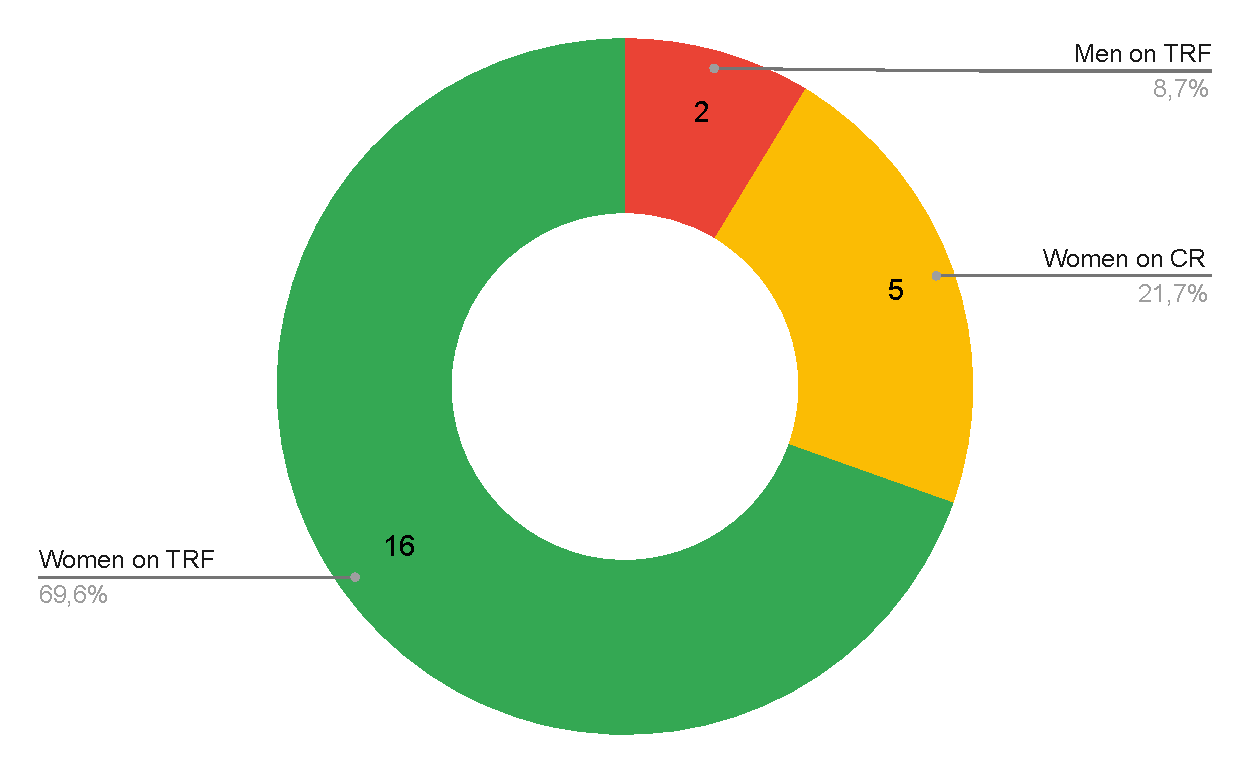
\includegraphics[width=10.5 cm]{Figure 1.pdf}
\caption{Patient distribution according to sex (Male and Female) and chosen nutritional intervention (TRF or CR).\label{fig1}}
\end{figure}   

Nutritional guidelines were made and personalized for each patient according to their group, following certain rules:
\\
\begin{itemize}
\item	The \textbf{TRF group} {\color{blue}followed a diet free of sugar and saturated fats, with caloric intake tailored to the patient's total energy expenditure. This was distributed over 8 hours of food intake and a 16-hour daily fast, adjusted to best fit their daily schedule}
\item	The \textbf{CR group} was based on the Obesity Society guidelines, with a total caloric intake 25\% less than total energy expenditure. This was distributed in 4 meals and 1 snack according to the following proportions: 55\% for carbohydrates, 15\% protein and 30\% fat, without sugar or saturated fat;
\end{itemize}

\subsection{Step 3: Monitoring}

Throughout the investigation, the following parameters were closely monitored:
\begin{itemize}
\item	\textbf{Treatment adherence:} patients were called once a week and important concepts related to their intervention were reinforced. A dairy registry was considered initially, but ultimately decided against due to the anxiety it generated in patients. 
\item	\textbf{Toxicity:} once a week during their consultation with radiation oncology, acute toxicity was assessed using the National Cancer Institute Common Terminology Criteria for Adverse Events (CTCAE);
\end{itemize}

\subsection{Step 4: Final Evaluation}

12 weeks after having started the intervention, and at least 4 weeks after finishing oncologic treatment, the following were measured:
\begin{itemize}
\item	Acute Toxicity;
\item	Weight and waist circumference;
\item	Fasting glucose, basal insulin and lipid profile;
\item	QoL with EORTC-c30, EORTC QLQ - BR23 (for breast cancer) and the EPIC 2.0 (for prostate cancer);
\end{itemize}
\section{Hypothesis}

CR or TRF are feasible and effective interventions in overweight and obese patients with breast or prostate cancer undergoing curative radiotherapy.\\
\section{Primary objectives}

Evaluate feasibility and effectiveness of CR and TRF in overweight and obese patients with cancer under curative radiotherapy.\\
\section{Secondary Objectives}

\begin{itemize}
\item	Assess adherence, defined as a reduction in body weight of at least 5\% compared to baseline and in at least 50\% of the recruited patients.;
\item	Establish which intervention (CR or TRF) has better adherence;
\item	Assess the impact on quality of life in patients under nutritional interventions;
\item	Assess differences in weight and waist circumference in patients under nutritional interventions;
\item	Assess differences in serum levels of fasting glucose, basal insulin and lipid profile in patients under nutritional interventions;
\item	Assess acute toxicity grade ≥2 in patients under nutritional interventions;
\end{itemize}

%%%%%%%%%%%%%%%%%%%%%%%%%%%%%%%%%%%%%%%%%%
\section{Results}

Descriptive statistics were used to characterize clinical and anthropometric data on the entire cohort. Variables with p value <0.05 were considered statistically significant. Statistical analyses were conducted with STATA/IC (version 16.1, StataCorp, College Station, USA).\\

27 patients were recruited from April 2021 to May 2023. Two patients withdrew from the trial before treatment and one patient did not receive radiotherapy (as seen in Figure~\ref{fig2}). At the end of May 2023, 23 patients had completed 12 weeks of follow up of which 21 were women and 2 were men. 

\begin{figure}[H]
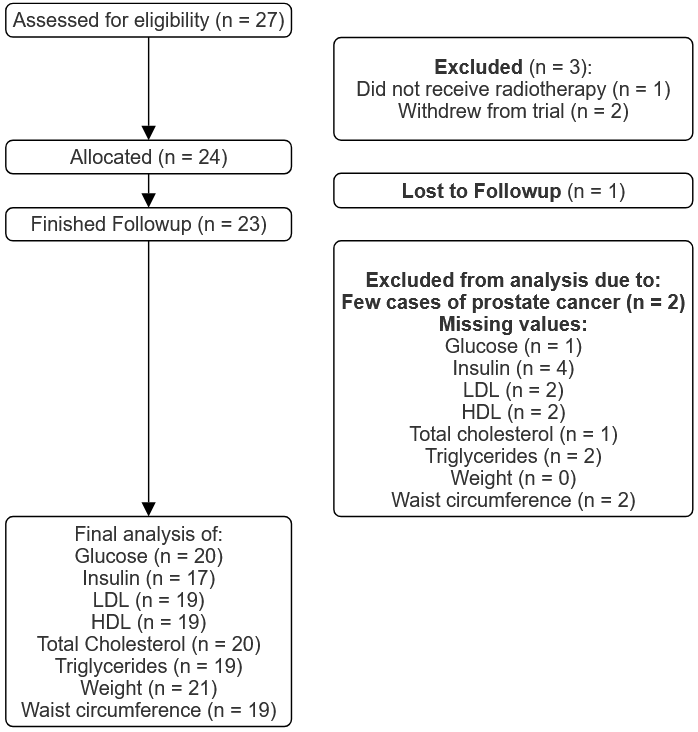
\includegraphics[width=10.5 cm]{Figure2.png}
\caption{\textbf{General outline of the study.} Diagram depicting steps and results yielded by the study.\label{fig2}}
\end{figure}   


Of the 23 patients available for analysis, 21 were women with breast cancer with luminal ductal carcinoma being the most common histologic subtype. From the 21 women with breast cancer, 14 received some kind of chemotherapy (neoadjuvant, adjuvant or both), and 19 received endocrine therapy. All 21 patients underwent whole breast radiotherapy (+-regional nodal irradiation) and 11 received simultaneous integrated boost to the tumor bed up to 45,75 Gy.\\

The remaining 2 patients were men with prostate cancer and a Gleason score of 6 and 7. Both of them underwent surgery and had initiated androgen deprivation therapy. They received  a dose of 51 Gy in 17 fractions to the prostate bed or equivalent EQD2. {\color{blue}However, they were left out of analysis due to insufficient scientific significance and difficulty interpreting results.}\\

{\color{blue}The following results were acquired from data available in Table~\ref{TablaMetab} and Table~\ref{TablaAnal}. Findings are described in the following paragraphs.

\begin{table}[h]
\centering
\caption{Analysis of the impact of TRF and CR on metabolic and anthropometrical parameters\label{TablaAnal}}
\begin{tabular}{lccccc}
\hline
\textbf{Parameter} & \textbf{Group} & \textbf{Mean Change} & \textbf{Std Dev} & \textbf{95\% CI} & \textbf{P-Value} \\
\hline
\multirow{2}{*}{Total Cholesterol} & CR & 10.27 & 28.11 & [-5.30, 25.83] & 0.179 \\
                                  & TRF & -6.4 & 42.09 & [-58.67, 45.87] & 0.751 \\
\hline
\multirow{2}{*}{Triglycerides}     & CR & 3.64 & 85.51 & [-45.73, 53.02] & 0.876 \\
                                  & TRF & 51 & 49.553 & [-10.53, 112.53] & 0.083 \\
\hline
\multirow{2}{*}{HDL}               & CR & 1.00 & 8.64 & [-5.99, 3.99] & 0.672 \\
                                  & TRF & -2 & 5.83 & [-9.24, 5.24] & 0.486 \\
\hline
\multirow{2}{*}{LDL}               & CR & -3.01 & 22.77 & [-10.13, 16.16] & 0.629 \\
                                  & TRF & -14.28 & 38.73 & [-62.37, 33.81] & 0.457 \\
\hline
\multirow{2}{*}{Weight}            & CR & 3.02 & 3.99 & [0.89, 5.15] & 0.009 \\
                                  & TRF & 6.84 & 3.85 & [2.05, 11.62] & 0.017 \\
\hline
\multirow{2}{*}{Waist Circumference} & CR & 4.14 & 5.67 & [0.87, 7.41] & 0.017 \\
                                    & TRF & 7.5 & 1.66 & [5.44, 9.55] & 0.004 \\
\hline
\multirow{2}{*}{Insulin}           & CR & 2.76 & 14.94 & [-6.26, 11.79] & 0.518 \\
                                  & TRF & -0.675 & 5.649 & [-9.66, 8.31] & 0.826 \\
\hline
\multirow{2}{*}{Glucose}           & CR & 1.81 & 8.30 & [-2.78, 6.41] & 0.412 \\
                                  & TRF & -1.6 & 5.90 & [-8.92, 5.72] & 0.577 \\
\hline
\end{tabular}
\end{table}


In this study, we evaluated the effects of Calorie Restriction (CR) and Time Restricted Feeding (TRF) on various health parameters within each group.\\

For Total Cholesterol, the CR group exhibited a nonsignificant mean increase (Mean Change = 10.27, CI = [-5.30, 25.83], P-Value = 0.179), while the TRF group showed a nonsignificant mean decrease (Mean Change = -6.4, CI = [-58.67, 45.87], P-Value = 0.751), indicating considerable variability in responses within both groups. Triglycerides levels in the CR group slightly increased (Mean Change = 3.64, CI = [-45.73, 53.02], P-Value = 0.876), whereas the TRF group showed a more substantial increase (Mean Change = 51, CI = [-10.53, 112.53], P-Value = 0.083), yet both were not statistically significant, \\

HDL changes were minimal and not significant in both groups (CR: Mean Change = 1.00, CI = [-5.99, 3.99], P-Value = 0.672; TRF: Mean Change = -2, CI = [-9.24, 5.24], P-Value = 0.486). LDL levels also did not show significant changes (CR: Mean Change = -3.01, CI = [-10.13, 16.16], P-Value = 0.629; TRF: Mean Change = -14.28, CI = [-62.37, 33.81], P-Value = 0.457).\\

Weight changes were significant in both groups, with the CR group losing an average of 3.02 kg (CI = [0.89, 5.15], P-Value = 0.009) and the TRF group 6.84 kg (CI = [2.05, 11.62], P-Value = 0.017), suggesting the effectiveness of both interventions in weight reduction. Waist Circumference also significantly decreased (CR: Mean Change = 4.14, CI = [0.87, 7.41], P-Value = 0.017; TRF: Mean Change = 7.5, CI = [5.44, 9.55], P-Value = 0.004).\\

For Insulin, changes were not significant in either group (CR: Mean Change = 2.76, CI = [-6.26, 11.79], P-Value = 0.518; TRF: Mean Change = -0.675, CI = [-9.66, 8.31], P-Value = 0.826). Similarly, Glucose levels did not exhibit significant changes (CR: Mean Change = 1.81, CI = [-2.78, 6.41], P-Value = 0.412; TRF: Mean Change = -1.6, CI = [-8.92, 5.72], P-Value = 0.577).\\

In conclusion, while both CR and TRF interventions were effective in reducing weight and waist circumference, their impact on lipid profile, glucose, and insulin levels were not significant. The variability within each parameter suggests a differential response to the dietary interventions.\\

Percentage analysis of data from Table~\ref{TablaMetab} and Table~\ref{TablaPorce} was done, giving the following results:\\

\begin{table}[ht]
\centering
\caption{Your Caption Here}
\label{TablaPorce}
\begin{tabular}{rlrrlll}
\toprule
 Age & Group &  Weight 1 &  Weight 2 &  \% Change &   WC 1 &   WC 2 \\
\midrule
 30 &    CR &      82.8 &      78.1 &  -5.68 &     91 &   86.0 \\
 34 &    CR &      70.0 &      63.0 & -10.00 &     84 &   79.0 \\
 67 &    CR &      83.5 &      89.0 &   6.59 &    107 &  116.0 \\
 43 &    CR &     103.0 &     100.0 &  -2.91 &      - &      - \\
 53 &    CR &      82.5 &      83.5 &   1.21 &    104 &  101.0 \\
 48 &    CR &      72.5 &      71.6 &  -1.24 &     93 &   93.5 \\
 70 &    CR &      72.3 &      63.5 & -12.17 &   97.5 &   88.0 \\
 58 &    CR &      77.0 &      75.0 &  -2.60 &    108 &  101.0 \\
 36 &    CR &      76.8 &      72.0 &  -6.25 &   85.5 &   81.0 \\
 49 &    CR &      86.2 &      86.0 &  -0.23 &   96.5 &   95.0 \\
 65 &    CR &      62.6 &      60.5 &  -3.35 &     88 &   85.0 \\
 43 &    CR &      84.0 &      73.3 & -12.74 &     98 &   90.5 \\
 60 &    CR &      71.0 &      66.0 &  -7.04 &     96 &      - \\
 47 &    CR &      67.0 &      68.0 &   1.49 &     89 &   90.0 \\
 60 &    CR &      81.2 &      77.0 &  -5.17 &    102 &   95.0 \\
 52 &    CR &      77.0 &      74.6 &  -3.12 &  107.5 &   92.0 \\
 49 &   TRF &      75.8 &      62.3 & -17.81 &     92 &   83.0 \\
 62 &   TRF &      66.5 &      61.0 &  -8.27 &    102 &   96.0 \\
 55 &   TRF &      70.0 &      66.0 &  -5.71 &     85 &   79.0 \\
 48 &   TRF &      77.4 &      72.8 &  -5.94 &     93 &   86.0 \\
 65 &   TRF &      76.1 &      69.5 &  -8.67 &   94.5 &   85.0 \\
\bottomrule
\end{tabular}
\footnotesize{This is a table footnote.}
\end{table}


\begin{itemize}
\item	There was a reported loss of 5\% or more of the initial weight (adherence) in 57,1\% of patients (12/21).
\item	100\% of those who chose TRF showed true adherence (5 out of 5), whereas only 43.75\% (7 out of 16) showed true adherence in the CR group.
\item	 of the 12 patients who showed true adherence, all 12 were women. 5 were on the TRF group (5 out of 7 patients in the TRF group) and 7 were on the CR group (7 out of 16 patients in the CR group). None of the men showed true adherence.
\end{itemize}
}
%%%%%%%%%%%%%%%%%%%%%%%%%%%%%%%%%%%%%%%%%%
\section{Discussion}

Our findings show that 57.1\% of patients lost 5\% or more of the initial weight, which shows that a nutrition intervention of these characteristics is not only feasible and attains true adherence from participants, but is also effective in reducing metabolic parameters in a short period of time (12 weeks).\\

Compared with other publications, our results are consistent with the available literature. TRF showed similar results to existing articles \cite{kalam2023intermittent}: high degree of adherence, decrease in weight, and improvement of blood glucose and insulin levels. Our differences in the result of blood glucose levels may be explained by the low adherence of both men in the TRF group. The differences with the study from Harvie \cite{harvie2022randomised} may be explained due to the fact they used another approach of IF which focuses on the amount of calories consumed (2 days of 650-1000 kcal/day before chemotherapy infusion) rather than the window of time they are consumed within.\\

Of interest is the differences of findings with the systematic review from Anemoulis et al. \cite{anemoulis2023intermittent}. This could be explained due to the type of IF approaches utilized in the studies considered, where only one of them specified the use of TRF, and the others were variations of calorie restricting approaches of IF: one included Ramadan-fasting patients, one used a FMD, while the others employed varied hours of fasting before and after chemotherapy. This reinforces the need for clear and established definitions of IF and its different approaches, and also an urgent necessity of evidence in this field.\\

Our findings are similar in adherence, weight loss and insulin levels in both interventions. We found that both TRF and CR managed to improve mean serum glucose, insulin, and TG levels. We also found that TRF was a vastly superior intervention in comparison to CR when it came to improving insulin and TG levels, but more research is required to further cement these findings in international literature.\\

Not only did these interventions as a group achieve true adherence, but 100\% of the patients with breast cancer in the TRF group showed true adherence in comparison to only 43.75\% adhering in the CR group, despite previous literature indicating breast cancer patients favored a CR approach \cite{kalam2023intermittent}.\\

We believe these findings to be due to how TRF does not restrict the amount of calories in a certain day, but rather restricts the timing of meals to 4 - 12 hours a day (8 hours in this study) and thus may be easier to carry on in cancer patients  busy with the whole therapeutic process. Further research is needed on this aspect.\\

Despite both interventions showing positive results, it seems TRF as a nutritional intervention has both better adherence, improved anthropometric values and metabolic serum levels.\\

In this novel clinical trial, we propose a straightforward and easy to replicate method with which to reclute patients and further study nutritional interventions besides TRF or CR, which we believe can provide the base for future nutritional intervention studies and open a window into other aspects of nutritional interventions such as impact on toxicity reduction which, although seen in animals \cite{cortellino2023fasting, de2019fasting}, has yet to be reproduced and further explored in human participants.\\

To our knowledge it is the first published work of this intervention in developing countries and showed consistent efficacy of the intervention.\\

\startlandscape
\begin{longtable}{|l|l|l|l|l|l|l|l|l|l|l|l|l|l|}
\caption{Your Caption Here}\label{TablaMetab} \\ % Caption and label

\hline
Age & Group & \multicolumn{2}{c|}{Total Cholesterol} & \multicolumn{2}{c|}{Triglycerides} & \multicolumn{2}{c|}{HDL} & \multicolumn{2}{c|}{LDL} & \multicolumn{2}{c|}{Insuline} & \multicolumn{2}{c|}{Glucose} \\ \hline
\endfirsthead % Header for the first page

\multicolumn{14}{c}%
{{\bfseries Table \thetable\ Continued from previous page}} \\
\hline
Age & Group & \multicolumn{2}{c|}{Total Cholesterol} & \multicolumn{2}{c|}{Triglycerides} & \multicolumn{2}{c|}{HDL} & \multicolumn{2}{c|}{LDL} & \multicolumn{2}{c|}{Insuline} & \multicolumn{2}{c|}{Glucose} \\ \hline
\endhead % Header for the remaining pages

% Repeat the headers for the last foot (optional)
\hline
\endfoot
 30 &    CR &                         176 &                    191.0 &                     143 &                296.0 &            43 &       44.0 &         105.0 &       87.0 &              15.3 & 21.9 &                91 &           84.0 \\
  34 &    CR &                         244 &                    214.0 &                     236 &                157.0 &            51 &       56.0 &         146.0 &      126.6 &               9.9 & 11.8 &                87 &           95.0 \\
  67 &    CR &                         204 &                    203.0 &                     174 &                137.0 &            38 &       43.0 &         132.0 &      132.0 &              10.0 & 11.6 &               106 &           96.0 \\
  43 &    CR &                         169 &                    207.0 &                     133 &                112.0 &            49 &       64.0 &          93.0 &      121.0 &              13.0 & 8.8 &                85 &           78.0 \\
  53 &    CR &                         158 &                    110.0 &                     428 &                317.0 &            37 &       37.0 &         121.0 &       99.0 &              43.2 &                47.8 &               108 &          112.0 \\
  48 &    CR &                         160 &                    137.0 &                     212 &                334.0 &            35 &       30.0 &          82.0 &       41.0 &              15.4 & 18.7 &               102 &          103.0 \\
  70 &    CR &                         149 &                    128.0 &                      77 &                 84.0 &            44 &       29.0 &          89.0 &       83.0 &              22.1 & 12.5 &               103 &          101.0 \\
  58 &    CR &                         182 &                    184.0 &                     241 &                228.0 &            38 &       34.0 &          96.0 &      104.0 &              10.0 & 11.9 &               106 &          113.0 \\
  36 &    CR &                         188 &                    202.0 &                      82 &                 68.0 &            67 &       82.0 &         105.0 &      106.0 &               5.4 & 4.7 &                87 &           92.0 \\
  49 &    CR &                         163 &                    171.0 &                      81 &                 90.0 &            60 &       58.0 &          86.0 &       95.0 &              15.3 & 18.1 &                96 &           91.0 \\
  65 &    CR &                         222 &                    188.0 &                     166 &                181.0 &            56 &       52.0 &         133.0 &       99.0 &               6.5 & 11.1 &                88 &           91.0 \\
  43 &    CR &                         204 &                    168.0 &                     356 &                179.0 &            22 &       26.0 &         111.0 &      107.0 &              67.8 & 17.3 &               102 &           85.0 \\
  60 &    CR &                         241 &                      ND &                     180 &                  ND &            60 &        NaN &         145.0 &        NaN &              11.6 &                 ND &                81 &            ND \\
  47 &    CR &                         244 &                    280.0 &                      76 &                127.0 &            56 &       65.0 &         172.8 &      189.0 &               7.8 &                 ND &                81 &           89.8 \\
  60 &    CR &                         230 &                    188.0 &                     360 &                404.0 &            43 &       33.0 &         115.0 &      155.0 &              13.6 & 15.4 &                91 &           75.0 \\
  52 &    CR &                         243 &                    211.0 &                     187 &                  ND &            67 &        NaN &         139.0 &        NaN &               9.3 &                 ND &                96 &           96.0 \\
  49 &   TRF &                         214 &                    167.0 &                     230 &                138.0 &            40 &       46.0 &         128.0 &       93.0 &              14.0 & 7.6 &                89 &           98.0 \\
  62 &   TRF &                         211 &                    241.0 &                     150 &                114.0 &            46 &       48.0 &         135.0 &      170.0 &              10.8 & 14.1 &                99 &          106.0 \\
  55 &   TRF &                         175 &                    183.0 &                     104 &                 87.0 &            54 &       60.0 &         100.0 &      105.0 &              10.1 & 9.2 &                92 &           89.0 \\
  48 &   TRF &                         192 &                    253.0 &                     132 &                135.0 &            48 &       40.0 &         117.6 &      185.0 &              15.3 &                  22 &               106 &          104.0 \\
  65 &   TRF &                         192 &                    172.0 &                     235 &                122.0 &            53 &       57.0 &          92.0 &       91.0 &               NaN & 13.4 &                94 &           91.0\footnotemark \\

\end{longtable}
\footnotesize{\textsuperscript{1} This is a table footnote.}
\finishlandscape

%%%%%%%%%%%%%%%%%%%%%%%%%%%%%%%%%%%%%%%%%%
\section{Limitations and Future Direction of Work}

{\color{blue}Limitations of our work are: small sample size and small power to detect differences in metabolic parameters, a relatively short period of surveillance, lack of adherence of patients to the guidelines given, limited generalization of study due to only recluting breast cancer patients, only evaluating the TRF approach of IF, lack of long term followup, and the absence of a control group.\\

This work could be improved by an increase in the number of patients, include QoL and acute toxicity to create a more holistic view of patient outcomes, include other cancer populations to further generalize our findings, increase the time of surveillance and include a period of followup, employing other nutritional interventions such as KD, alternate day fasting or FMD to better compare results between interventions, measuring blood levels of inflammatory response markers, measuring blood levels of hormonal markers, measure fat mass and lean mass percentages, the inclusion of a control group, or the incorporation of feedback from participants.\\

We believe these factors are a must to be taken to ensure robust findings. Once international consensus is achieved between the different definitions and approaches of the various nutritional interventions and a strong methodology is properly built and assured, future research should look to apply these conditions on different cohorts to better generalize these findings and eventually include them in international guidelines.}


%%%%%%%%%%%%%%%%%%%%%%%%%%%%%%%%%%%%%%%%%%
\section{Conclusions}

Cardiovascular diseases and cancer lead incidence and mortality rates worldwide, sharing common risk factors such as overweight and obesity. These play an important role in the origin of breast and prostate cancer, and thus different interventions have been investigated to establish a faithful and reproducible way {\color{blue}to achieve weight loss} in cancer patients.\\

The theory behind the benefit of diet and weight loss in cancer has been largely studied and established in preclinical studies, but clinical studies that show these results in practice are few in between and limited in their approach. This could be attributed to the numerous interventions in existence and a lack of agreement on definitions, establishing which ones are best, and also a lack of patients on which these interventions have been measured thoroughly.\\

{\color{blue}Two of these interventions are TRF and CR. These nutritional interventions were chosen in this study due to their historical relevance and evidence supporting them. Our findings are consistent with the literature. Both CR and TRF achieve a statistically significant loss of weight and reduction in waist circumference, but TRF shows a larger effect size and larger average change in both weight loss and reduction in waist circumference. Changes in metabolic parameters were not statistically significant.}\\

Differences with literature can be explained due to heterogeneity on application of IF and its different approaches, lacking a formal definition. This leads to large differences in fasting hours, number of fasting days and the existence or not of a caloric restriction.\\

We propose a series of steps through which metabolic parameters, anthropometry and quality of life can be measured. These steps are simple to apply and reproducible. We hope this helps establish concrete and well established definitions of the various fasting regimes, and motivates other researchers to further investigate and build the foundation of what we believe is a low-cost and effective way to lose weight and improve metabolic parameters.\\


\printbibliography

%%%%%%%%%%%%%%%%%%%%%%%%%%%%%%%%%%%%%%%%%%

%%%%%%%%%%%%%%%%%%%%%%%%%%%%%%%%%%%%%%%%%%
\vspace{6pt} 

%%%%%%%%%%%%%%%%%%%%%%%%%%%%%%%%%%%%%%%%%%
%% optional



%%%%%%%%%%%%%%%%%%%%%%%%%%%%%%%%%%%%%%%%%%
\supplementary{The following supporting information has been uploaded together with the manuscript: Supplementary Spreadsheet 1: 24- hour Reminder Survey.}

\authorcontributions{Conceptualization, Carmen Vega and Tomás Merino; Data curation, Esteban Barnafi and Nicolás Rivas; Funding acquisition, Carmen Vega; Investigation, Carmen Vega, Alejandra Parada and Nicolás Rivas; Methodology, Carmen Vega and Tomás Merino; Project administration, Carmen Vega; Resources, César Sánchez, Francisco Acevedo, Benjamin Walbaum and Tomás Merino; Supervision, Carmen Vega and Francisco Acevedo; Validation, Tomás Merino; Visualization, Esteban Barnafi; Writing – original draft, Esteban Barnafi; Writing – review & editing, Carmen Vega, Esteban Barnafi and Tomás Merino.}

\funding{This research was funded by CONCURSO DE INVESTIGACIÓN PARA RESIDENTES DE POSGRADO, ESCUELA DE MEDICINA, FACULTAD DE MEDICINA, PONTIFICIA UNIVERSIDAD CATÓLICA DE CHILE. }

\institutionalreview{This study was conducted with the approval of the Comité Ético Científico de Ciencias de la Salud UC (CEC-Salud UC). This Committee adheres to the ethical principles of Pontificia Universidad Católica de Chile, which considers respect for the dignity of the human person in any condition as a fundamental axis. This Committee also complies with the Good Clinical Practice Guidelines defined by the International Conference on Harmonization (GCP-ICH); and with Chilean laws 19.628; 20.120; 20.584 and 20.850 that modify the Health Code.}

\informedconsent{Written informed consent was obtained from all subjects involved in the study after the procedure and the steps involved were explained.}

\dataavailability{All statements and conclusions made within this article have been made with the data and information contained within the provided supplements (tables and figures). No other data was used.} 

% Only for journal Nursing Reports
%\publicinvolvement{Please describe how the public (patients, consumers, carers) were involved in the research. Consider reporting against the GRIPP2 (Guidance for Reporting Involvement of Patients and the Public) checklist. If the public were not involved in any aspect of the research add: ``No public involvement in any aspect of this research''.}

% Only for journal Nursing Reports
%\guidelinesstandards{Please add a statement indicating which reporting guideline was used when drafting the report. For example, ``This manuscript was drafted against the XXX (the full name of reporting guidelines and citation) for XXX (type of research) research''. A complete list of reporting guidelines can be accessed via the equator network: \url{https://www.equator-network.org/}.}

\acknowledgments{We kindly thank N.B for his relentless revisions and support during the manufacturing of this manuscript.}

\conflictsofinterest{The authors declare no conflict of interest. The funders had no role in the design of the study; in the collection, analyses, or interpretation of data; in the writing of the manuscript; or in the decision to publish the results.} 

%%%%%%%%%%%%%%%%%%%%%%%%%%%%%%%%%%%%%%%%%%
%% Optional

%% Only for journal Encyclopedia
%\entrylink{The Link to this entry published on the encyclopedia platform.}

\abbreviations{Abbreviations}{
The following abbreviations are used in this manuscript:\\

\noindent 
\begin{tabular}{@{}ll}
MDPI & Multidisciplinary Digital Publishing Institute\\
DOAJ & Directory of open access journals\\
TLA & Three letter acronym\\
LD & Linear dichroism
\end{tabular}
}

%%%%%%%%%%%%%%%%%%%%%%%%%%%%%%%%%%%%%%%%%%
%% Optional
\appendixtitles{no} % Leave argument "no" if all appendix headings stay EMPTY (then no dot is printed after "Appendix A"). If the appendix sections contain a heading then change the argument to "yes".
\appendixstart
\appendix
\section[\appendixname~\thesection]{}
\subsection[\appendixname~\thesubsection]{}
The appendix is an optional section that can contain details and data supplemental to the main text---for example, explanations of experimental details that would disrupt the flow of the main text but nonetheless remain crucial to understanding and reproducing the research shown; figures of replicates for experiments of which representative data are shown in the main text can be added here if brief, or as Supplementary Data. Mathematical proofs of results not central to the paper can be added as an appendix.

\begin{table}[H] 
\caption{This is a table caption.\label{tab5}}
\newcolumntype{C}{>{\centering\arraybackslash}X}
\begin{tabularx}{\textwidth}{CCC}
\toprule
\textbf{Title 1}	& \textbf{Title 2}	& \textbf{Title 3}\\
\midrule
Entry 1		& Data			& Data\\
Entry 2		& Data			& Data\\
\bottomrule
\end{tabularx}
\end{table}

\section[\appendixname~\thesection]{}
All appendix sections must be cited in the main text. In the appendices, Figures, Tables, etc. should be labeled, starting with ``A''---e.g., Figure A1, Figure A2, etc.

%%%%%%%%%%%%%%%%%%%%%%%%%%%%%%%%%%%%%%%%%%
\begin{adjustwidth}{-\extralength}{0cm}
%\printendnotes[custom] % Un-comment to print a list of endnotes

\reftitle{References}

% Please provide either the correct journal abbreviation (e.g. according to the “List of Title Word Abbreviations” http://www.issn.org/services/online-services/access-to-the-ltwa/) or the full name of the journal.
% Citations and References in Supplementary files are permitted provided that they also appear in the reference list here. 

%=====================================
% References, variant A: external bibliography
%=====================================
%\bibliography{your_external_BibTeX_file}

%=====================================
% References, variant B: internal bibliography
%=====================================
\begin{thebibliography}{999}
% Reference 1
\bibitem[Author1(year)]{ref-journal}
Author~1, T. The title of the cited article. {\em Journal Abbreviation} {\bf 2008}, {\em 10}, 142--149.
% Reference 2
\bibitem[Author2(year)]{ref-book1}
Author~2, L. The title of the cited contribution. In {\em The Book Title}; Editor 1, F., Editor 2, A., Eds.; Publishing House: City, Country, 2007; pp. 32--58.
% Reference 3
\bibitem[Author3(year)]{ref-book2}
Author 1, A.; Author 2, B. \textit{Book Title}, 3rd ed.; Publisher: Publisher Location, Country, 2008; pp. 154--196.
% Reference 4
\bibitem[Author4(year)]{ref-unpublish}
Author 1, A.B.; Author 2, C. Title of Unpublished Work. \textit{Abbreviated Journal Name} year, \textit{phrase indicating stage of publication (submitted; accepted; in press)}.
% Reference 5
\bibitem[Author5(year)]{ref-communication}
Author 1, A.B. (University, City, State, Country); Author 2, C. (Institute, City, State, Country). Personal communication, 2012.
% Reference 6
\bibitem[Author6(year)]{ref-proceeding}
Author 1, A.B.; Author 2, C.D.; Author 3, E.F. Title of presentation. In Proceedings of the Name of the Conference, Location of Conference, Country, Date of Conference (Day Month Year); Abstract Number (optional), Pagination (optional).
% Reference 7
\bibitem[Author7(year)]{ref-thesis}
Author 1, A.B. Title of Thesis. Level of Thesis, Degree-Granting University, Location of University, Date of Completion.
% Reference 8
\bibitem[Author8(year)]{ref-url}
Title of Site. Available online: URL (accessed on Day Month Year).
\end{thebibliography}

% If authors have biography, please use the format below
%\section*{Short Biography of Authors}
%\bio
%{\raisebox{-0.35cm}{\includegraphics[width=3.5cm,height=5.3cm,clip,keepaspectratio]{Definitions/author1.pdf}}}
%{\textbf{Firstname Lastname} Biography of first author}
%
%\bio
%{\raisebox{-0.35cm}{\includegraphics[width=3.5cm,height=5.3cm,clip,keepaspectratio]{Definitions/author2.jpg}}}
%{\textbf{Firstname Lastname} Biography of second author}

% For the MDPI journals use author-date citation, please follow the formatting guidelines on http://www.mdpi.com/authors/references
% To cite two works by the same author: \citeauthor{ref-journal-1a} (\citeyear{ref-journal-1a}, \citeyear{ref-journal-1b}). This produces: Whittaker (1967, 1975)
% To cite two works by the same author with specific pages: \citeauthor{ref-journal-3a} (\citeyear{ref-journal-3a}, p. 328; \citeyear{ref-journal-3b}, p.475). This produces: Wong (1999, p. 328; 2000, p. 475)

%%%%%%%%%%%%%%%%%%%%%%%%%%%%%%%%%%%%%%%%%%
%% for journal Sci
%\reviewreports{\\
%Reviewer 1 comments and authors’ response\\
%Reviewer 2 comments and authors’ response\\
%Reviewer 3 comments and authors’ response
%}
%%%%%%%%%%%%%%%%%%%%%%%%%%%%%%%%%%%%%%%%%%
\PublishersNote{}
\end{adjustwidth}
\end{document}

